


\section{Restriction}
	In our implementation we first cycle through all of the true coarse grid points, then
	the two main tasks is to find the specific fine grid point corresponding to the specific
 	coarse grid point, and finding the indexes of the fine grid points surrounding the grid point.

	Since the value in both grids are stored in a first order lexicographical array, we should treat the
	grid points in the same fashion, so the values are stored close to each other in the array.
	The first dimension is treated first, then the next is dimension is incremented followed by
	treating the first dimension again, then increment the next and so on. The fine grid has twice the
	resolution of the coarse grid, so for each time the coarse grid index is incremented,
	the fine grid index is incremented twice.

	Along the x-axis each incrementation is the number of values stored in the grid, which for scalars
	is \(1\), and 2 for the fine index. The fine index will in addition
	need to skip 1 row each time, each time the y-axis is incremented, due to the finer resolution and 1 layer each time
	the z-axis is incremented.

	At the edges of the grid we have ghost layers, which have equal thickness for both the grids, so the
	coarse grid needs to increment over the ghost values, in the x-direction, each time y is incremented.
	When z is incremented the index need to skip over a row of ghost values. The fine index follows
	the same procedure as the coarse index when dealing with the ghost layers.

	When correct fine grid index is found, corresponding to a coarse grid index, the stencil needs to be applied around
 	that grid value. This is done by first calculating the index of the first coarse and find indexes and setting
	the correct indexes for the surrounding grid values, then the surrounding grid indexes can be incremented
	exactly as the fine grid index and they will keep their shape around the fine grid index. Since our indexes
	in x, y and z are labeled j,l,k, the next value along the x-axis is labeled 'fj' and the previous is labeled
	'fjj'. The coarse and fine grid indexes are label 'c' and 'f' respectively.


\section{Prolongation}


	%Citation Numerical Recipes in C
	The algorithm implemented for the interpolation is based on the method, described in
	\cite{press_numerical_1988}, has the following steps, which is also shown for a 2D case in \ref{fig:prolongation}.

 	\begin{enumerate}
		\item Direct insertion: Coarse$\rightarrow$ Fine
		\item Interpolation on highest Dimension: \(f(x) = \frac{f(x+h) + f(x-h)}{2h}\)
		\item Fill needed ghosts.
		\item Interpolation on next highest Dimension
	\end{enumerate}

	The interpolation should always first be done on the highest dimension, because the grid values are stored further
	apart along the highest axis in the memory, and the each succesive interpolation needs to apply to more grid points. (Note to self: should test)

	%%%%%%%%%%%%%%%%%%%%%%%%%%%%%%%%%%%%%%%%%%%%%%%%%%%%%%%%%%%%%%%%%%%%%%%%%%%%%%%%%%%%5
	%%%		Tikz picture
	%%%%%%%%%%%%%%%%%%%%%%%%%%%%%%%%%%%%%%%%%%%%%%%%%%%%%%%%%%%%%%%%%%%%%%%%%%%%%%%%%%%%
	\tikzstyle{vertex}=[circle,fill=blue!40,minimum size=10pt,inner sep=0pt]
	\tikzstyle{ghost}=[circle,fill=blue!20,minimum size=10pt,inner sep=0pt]
	\tikzstyle{whole}=[circle, fill=black!100, minimum size = 10pt, inner sep=0pt]
	\tikzstyle{half}=[circle, fill=black!50, minimum size = 10pt, inner sep=0pt]
	\tikzstyle{quarter}=[circle, fill=black!25, minimum size = 10pt, inner sep=0pt]


	%Note to self: This should really have been done in a more automated/smarter way
	\begin{figure}
		\centering
		\begin{subfigure}[b]{0.45\textwidth}
		\centering
		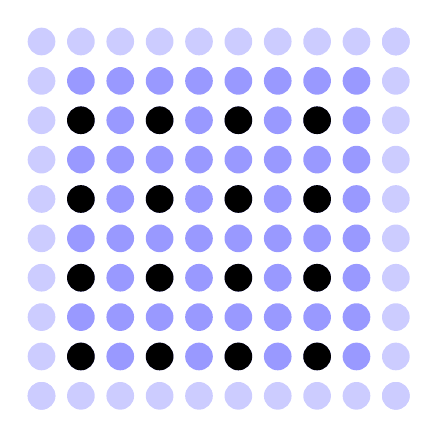
\begin{tikzpicture}[scale=0.50, auto,swap]
			%Adding the ghost nodes along the edges
			\foreach \pos/\name in 	{{(0,0)/},	{(1,0)/}, 	{(2,0)/},	{(3,0)/},
									 {(4,0)/},	{(5,0)/}, 	{(6,0)/},	{(7,0)/},
									 {(8,0)/},	{(9,0)/}}
			\node[ghost] (\name) at \pos {$\name$};
			\foreach \pos/\name in 	{			{(0,1)/}, 	{(0,2)/},		{(0,3)/},
									{(0,4)/},	{(0,5)/}, 	{(0,6)/},		{(0,7)/},
									{(0,8)/}, 	{(0,9)/}}
			\node[ghost] (\name) at \pos {$\name$};
			\foreach \pos/\name in 	{{(0,0)/},	{(1,9)/}, 	{(2,9)/},		{(3,9)/},
									 {(4,9)/},	{(5,9)/}, 	{(6,9)/},		{(7,9)/},
									 {(8,9)/}, 	{(9,9)/}}
			\node[ghost] (\name) at \pos {$\name$};
			\foreach \pos/\name in 	{{(9,0)/},	{(9,1)/}, {(9,2)/},		{(9,3)/},
									 {(9,4)/},	{(9,5)/}, {(9,6)/},		{(9,7)/},
									 {(9,8)/},	{(9,9)/}}
			\node[ghost] (\name) at \pos {$\name$};
			%The inner nodes
			\foreach \pos/\name in {{(1,1)/}, 	{(1,2)/},		{(1,3)/},		{(1,4)/},
									{(1,5)/}, 	{(1,6)/},		{(1,7)/},		{(1,8)/}}
			\node[vertex] (\name) at \pos {$\name$};
			\foreach \pos/\name in {{(2,1)/}, 	{(2,2)/},		{(2,3)/},		{(2,4)/},
									{(2,5)/}, 	{(2,6)/},		{(2,7)/},		{(2,8)/}}
			\node[vertex] (\name) at \pos {$\name$};
			\foreach \pos/\name in {{(3,1)/}, 	{(3,2)/},		{(3,3)/},		{(3,4)/},
									{(3,5)/}, 	{(3,6)/},		{(3,7)/},		{(3,8)/}}
			\node[vertex] (\name) at \pos {$\name$};
			\foreach \pos/\name in {{(4,1)/}, 	{(4,2)/},		{(4,3)/},		{(4,4)/},
									{(4,5)/}, 	{(4,6)/},		{(4,7)/},		{(4,8)/}}
			\node[vertex] (\name) at \pos {$\name$};
			\foreach \pos/\name in {{(5,1)/}, 	{(5,2)/},		{(5,3)/},		{(5,4)/},
									{(5,5)/}, 	{(5,6)/},		{(5,7)/},		{(5,8)/}}
			\node[vertex] (\name) at \pos {$\name$};
			\foreach \pos/\name in {{(6,1)/}, 	{(6,2)/},		{(6,3)/},		{(6,4)/},
									{(6,5)/}, 	{(6,6)/},		{(6,7)/},		{(6,8)/}}
			\node[vertex] (\name) at \pos {$\name$};
			\foreach \pos/\name in 	{{(7,1)/}, 	{(7,2)/},		{(7,3)/},		{(7,4)/},
									{(7,5)/}, 	{(7,6)/},		{(7,7)/},		{(7,8)/}}
			\node[vertex] (\name) at \pos {$\name$};
			\foreach \pos/\name in 	{{(8,1)/}, 	{(8,2)/},		{(8,3)/},		{(8,4)/},
									{(8,5)/}, 	{(8,6)/},		{(8,7)/},		{(8,8)/}}
			\node[vertex] (\name) at \pos {$\name$};
			%Adding direct insertion
			\foreach \pos/\name in 	{{(1,1)/}, 	{(3,1)/},		{(5,1)/},		{(7,1)/},
									 {(1,3)/}, 	{(3,3)/},		{(5,3)/},		{(7,3)/},
									 {(1,5)/}, 	{(3,5)/},		{(5,5)/},		{(7,5)/},
									 {(1,7)/}, 	{(3,7)/},		{(5,7)/},		{(7,7)/}}
			\node[whole] (\name) at \pos {$\name$};
		\end{tikzpicture}
		\caption{Direct insertion}
		\label{fig:direct}
		\end{subfigure}
		\centering
		\begin{subfigure}[b]{0.45\textwidth}
		\centering
		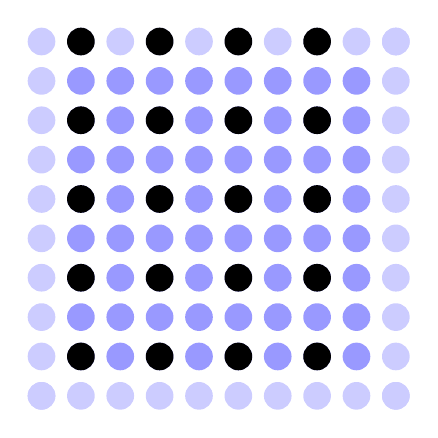
\begin{tikzpicture}[scale=0.50, auto,swap]
			%Adding the ghost nodes along the edges
			\foreach \pos/\name in 	{{(0,0)/},	{(1,0)/}, 	{(2,0)/},	{(3,0)/},
									 {(4,0)/},	{(5,0)/}, 	{(6,0)/},	{(7,0)/},
									 {(8,0)/},	{(9,0)/}}
			\node[ghost] (\name) at \pos {$\name$};
			\foreach \pos/\name in 	{			{(0,1)/}, 	{(0,2)/},		{(0,3)/},
									{(0,4)/},	{(0,5)/}, 	{(0,6)/},		{(0,7)/},
									{(0,8)/}, 	{(0,9)/}}
			\node[ghost] (\name) at \pos {$\name$};
			\foreach \pos/\name in 	{{(0,0)/},	{(1,9)/}, 	{(2,9)/},		{(3,9)/},
									 {(4,9)/},	{(5,9)/}, 	{(6,9)/},		{(7,9)/},
									 {(8,9)/}, 	{(9,9)/}}
			\node[ghost] (\name) at \pos {$\name$};
			\foreach \pos/\name in 	{{(9,0)/},	{(9,1)/}, {(9,2)/},		{(9,3)/},
									 {(9,4)/},	{(9,5)/}, {(9,6)/},		{(9,7)/},
									 {(9,8)/},	{(9,9)/}}
			\node[ghost] (\name) at \pos {$\name$};
			%The inner nodes
			\foreach \pos/\name in {{(1,1)/}, 	{(1,2)/},		{(1,3)/},		{(1,4)/},
									{(1,5)/}, 	{(1,6)/},		{(1,7)/},		{(1,8)/}}
			\node[vertex] (\name) at \pos {$\name$};
			\foreach \pos/\name in {{(2,1)/}, 	{(2,2)/},		{(2,3)/},		{(2,4)/},
									{(2,5)/}, 	{(2,6)/},		{(2,7)/},		{(2,8)/}}
			\node[vertex] (\name) at \pos {$\name$};
			\foreach \pos/\name in {{(3,1)/}, 	{(3,2)/},		{(3,3)/},		{(3,4)/},
									{(3,5)/}, 	{(3,6)/},		{(3,7)/},		{(3,8)/}}
			\node[vertex] (\name) at \pos {$\name$};
			\foreach \pos/\name in {{(4,1)/}, 	{(4,2)/},		{(4,3)/},		{(4,4)/},
									{(4,5)/}, 	{(4,6)/},		{(4,7)/},		{(4,8)/}}
			\node[vertex] (\name) at \pos {$\name$};
			\foreach \pos/\name in {{(5,1)/}, 	{(5,2)/},		{(5,3)/},		{(5,4)/},
									{(5,5)/}, 	{(5,6)/},		{(5,7)/},		{(5,8)/}}
			\node[vertex] (\name) at \pos {$\name$};
			\foreach \pos/\name in {{(6,1)/}, 	{(6,2)/},		{(6,3)/},		{(6,4)/},
									{(6,5)/}, 	{(6,6)/},		{(6,7)/},		{(6,8)/}}
			\node[vertex] (\name) at \pos {$\name$};
			\foreach \pos/\name in 	{{(7,1)/}, 	{(7,2)/},		{(7,3)/},		{(7,4)/},
									{(7,5)/}, 	{(7,6)/},		{(7,7)/},		{(7,8)/}}
			\node[vertex] (\name) at \pos {$\name$};
			\foreach \pos/\name in 	{{(8,1)/}, 	{(8,2)/},		{(8,3)/},		{(8,4)/},
									{(8,5)/}, 	{(8,6)/},		{(8,7)/},		{(8,8)/}}
			\node[vertex] (\name) at \pos {$\name$};
			%Adding direct insertion
			\foreach \pos/\name in 	{{(1,1)/}, 	{(3,1)/},		{(5,1)/},		{(7,1)/},
									 {(1,3)/}, 	{(3,3)/},		{(5,3)/},		{(7,3)/},
									 {(1,5)/}, 	{(3,5)/},		{(5,5)/},		{(7,5)/},
									 {(1,7)/}, 	{(3,7)/},		{(5,7)/},		{(7,7)/}}
			\node[whole] (\name) at \pos {$\name$};
			%X-Ghosts
			\foreach \pos/\name in 	{{(1,9)/}, 	{(3,9)/},		{(5,9)/},		{(7,9)/}}
			\node[whole] (\name) at \pos {$\name$};
		\end{tikzpicture}
		\caption{Swapping X-Dim ghosts}
		\label{fig:x_ghosts}
		\end{subfigure}
		\centering
		\begin{subfigure}[b]{0.45\textwidth}
		\centering
		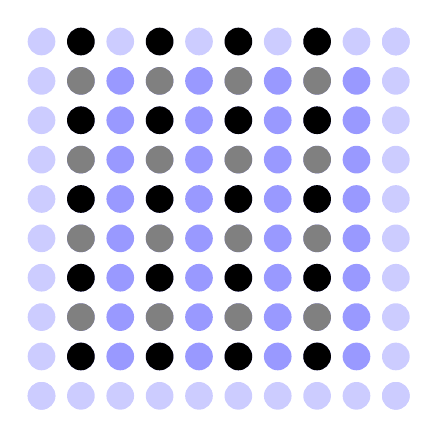
\begin{tikzpicture}[scale=0.5, auto,swap]
			%Adding the ghost nodes along the edges
			\foreach \pos/\name in 	{{(0,0)/},	{(1,0)/}, 	{(2,0)/},	{(3,0)/},
									 {(4,0)/},	{(5,0)/}, 	{(6,0)/},	{(7,0)/},
									 {(8,0)/},	{(9,0)/}}
			\node[ghost] (\name) at \pos {$\name$};
			\foreach \pos/\name in 	{			{(0,1)/}, 	{(0,2)/},		{(0,3)/},
									{(0,4)/},	{(0,5)/}, 	{(0,6)/},		{(0,7)/},
									{(0,8)/}, 	{(0,9)/}}
			\node[ghost] (\name) at \pos {$\name$};
			\foreach \pos/\name in 	{{(0,0)/},	{(1,9)/}, 	{(2,9)/},		{(3,9)/},
									 {(4,9)/},	{(5,9)/}, 	{(6,9)/},		{(7,9)/},
									 {(8,9)/}, 	{(9,9)/}}
			\node[ghost] (\name) at \pos {$\name$};
			\foreach \pos/\name in 	{{(9,0)/},	{(9,1)/}, {(9,2)/},		{(9,3)/},
									 {(9,4)/},	{(9,5)/}, {(9,6)/},		{(9,7)/},
									 {(9,8)/},	{(9,9)/}}
			\node[ghost] (\name) at \pos {$\name$};
			%The inner nodes
			\foreach \pos/\name in {{(1,1)/}, 	{(1,2)/},		{(1,3)/},		{(1,4)/},
									{(1,5)/}, 	{(1,6)/},		{(1,7)/},		{(1,8)/}}
			\node[vertex] (\name) at \pos {$\name$};
			\foreach \pos/\name in {{(2,1)/}, 	{(2,2)/},		{(2,3)/},		{(2,4)/},
									{(2,5)/}, 	{(2,6)/},		{(2,7)/},		{(2,8)/}}
			\node[vertex] (\name) at \pos {$\name$};
			\foreach \pos/\name in {{(3,1)/}, 	{(3,2)/},		{(3,3)/},		{(3,4)/},
									{(3,5)/}, 	{(3,6)/},		{(3,7)/},		{(3,8)/}}
			\node[vertex] (\name) at \pos {$\name$};
			\foreach \pos/\name in {{(4,1)/}, 	{(4,2)/},		{(4,3)/},		{(4,4)/},
									{(4,5)/}, 	{(4,6)/},		{(4,7)/},		{(4,8)/}}
			\node[vertex] (\name) at \pos {$\name$};
			\foreach \pos/\name in {{(5,1)/}, 	{(5,2)/},		{(5,3)/},		{(5,4)/},
									{(5,5)/}, 	{(5,6)/},		{(5,7)/},		{(5,8)/}}
			\node[vertex] (\name) at \pos {$\name$};
			\foreach \pos/\name in {{(6,1)/}, 	{(6,2)/},		{(6,3)/},		{(6,4)/},
									{(6,5)/}, 	{(6,6)/},		{(6,7)/},		{(6,8)/}}
			\node[vertex] (\name) at \pos {$\name$};
			\foreach \pos/\name in 	{{(7,1)/}, 	{(7,2)/},		{(7,3)/},		{(7,4)/},
									{(7,5)/}, 	{(7,6)/},		{(7,7)/},		{(7,8)/}}
			\node[vertex] (\name) at \pos {$\name$};
			\foreach \pos/\name in 	{{(8,1)/}, 	{(8,2)/},		{(8,3)/},		{(8,4)/},
									{(8,5)/}, 	{(8,6)/},		{(8,7)/},		{(8,8)/}}
			\node[vertex] (\name) at \pos {$\name$};
			%Adding direct insertion
			\foreach \pos/\name in 	{{(1,1)/}, 	{(3,1)/},		{(5,1)/},		{(7,1)/},
									 {(1,3)/}, 	{(3,3)/},		{(5,3)/},		{(7,3)/},
									 {(1,5)/}, 	{(3,5)/},		{(5,5)/},		{(7,5)/},
									 {(1,7)/}, 	{(3,7)/},		{(5,7)/},		{(7,7)/}}
			\node[whole] (\name) at \pos {$\name$};
			%X-Ghosts
			\foreach \pos/\name in 	{{(1,9)/}, 	{(3,9)/},		{(5,9)/},		{(7,9)/}}
			\node[whole] (\name) at \pos {$\name$};
			%Y-Swipe
			\foreach \pos/\name in 	{{(1,2)/}, 	{(3,2)/},		{(5,2)/},		{(7,2)/},
									 {(1,4)/}, 	{(3,4)/},		{(5,4)/},		{(7,4)/},
									 {(1,6)/}, 	{(3,6)/},		{(5,6)/},		{(7,6)/},
									 {(1,8)/}, 	{(3,8)/},		{(5,8)/},		{(7,8)/}}
			\node[half] (\name) at \pos {$\name$};
		\end{tikzpicture}
		\caption{Y-swipe\\\color{white}Lazy fix}
		\label{fig:y_swipe}
		\end{subfigure}
		\begin{subfigure}[b]{0.45\textwidth}
		\centering
		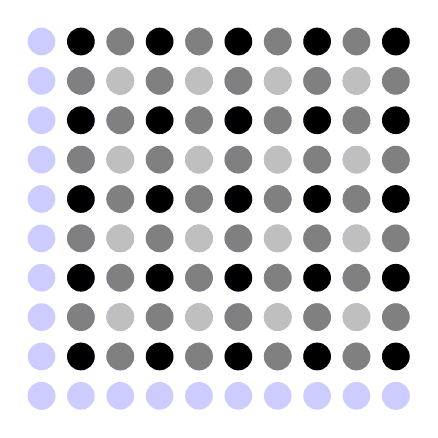
\begin{tikzpicture}[scale=0.5, auto,swap]
			%Adding the ghost nodes along the edges
			\foreach \pos/\name in 	{{(0,0)/},	{(1,0)/}, 	{(2,0)/},	{(3,0)/},
									 {(4,0)/},	{(5,0)/}, 	{(6,0)/},	{(7,0)/},
									 {(8,0)/},	{(9,0)/}}
			\node[ghost] (\name) at \pos {$\name$};
			\foreach \pos/\name in 	{			{(0,1)/}, 	{(0,2)/},		{(0,3)/},
									{(0,4)/},	{(0,5)/}, 	{(0,6)/},		{(0,7)/},
									{(0,8)/}, 	{(0,9)/}}
			\node[ghost] (\name) at \pos {$\name$};
			\foreach \pos/\name in 	{{(0,0)/},	{(1,9)/}, 	{(2,9)/},		{(3,9)/},
									 {(4,9)/},	{(5,9)/}, 	{(6,9)/},		{(7,9)/},
									 {(8,9)/}, 	{(9,9)/}}
			\node[ghost] (\name) at \pos {$\name$};
			\foreach \pos/\name in 	{{(9,0)/},	{(9,1)/}, {(9,2)/},		{(9,3)/},
									 {(9,4)/},	{(9,5)/}, {(9,6)/},		{(9,7)/},
									 {(9,8)/},	{(9,9)/}}
			\node[ghost] (\name) at \pos {$\name$};
			%The inner nodes
			\foreach \pos/\name in {{(1,1)/}, 	{(1,2)/},		{(1,3)/},		{(1,4)/},
									{(1,5)/}, 	{(1,6)/},		{(1,7)/},		{(1,8)/}}
			\node[vertex] (\name) at \pos {$\name$};
			\foreach \pos/\name in {{(2,1)/}, 	{(2,2)/},		{(2,3)/},		{(2,4)/},
									{(2,5)/}, 	{(2,6)/},		{(2,7)/},		{(2,8)/}}
			\node[vertex] (\name) at \pos {$\name$};
			\foreach \pos/\name in {{(3,1)/}, 	{(3,2)/},		{(3,3)/},		{(3,4)/},
									{(3,5)/}, 	{(3,6)/},		{(3,7)/},		{(3,8)/}}
			\node[vertex] (\name) at \pos {$\name$};
			\foreach \pos/\name in {{(4,1)/}, 	{(4,2)/},		{(4,3)/},		{(4,4)/},
									{(4,5)/}, 	{(4,6)/},		{(4,7)/},		{(4,8)/}}
			\node[vertex] (\name) at \pos {$\name$};
			\foreach \pos/\name in {{(5,1)/}, 	{(5,2)/},		{(5,3)/},		{(5,4)/},
									{(5,5)/}, 	{(5,6)/},		{(5,7)/},		{(5,8)/}}
			\node[vertex] (\name) at \pos {$\name$};
			\foreach \pos/\name in {{(6,1)/}, 	{(6,2)/},		{(6,3)/},		{(6,4)/},
									{(6,5)/}, 	{(6,6)/},		{(6,7)/},		{(6,8)/}}
			\node[vertex] (\name) at \pos {$\name$};
			\foreach \pos/\name in 	{{(7,1)/}, 	{(7,2)/},		{(7,3)/},		{(7,4)/},
									{(7,5)/}, 	{(7,6)/},		{(7,7)/},		{(7,8)/}}
			\node[vertex] (\name) at \pos {$\name$};
			\foreach \pos/\name in 	{{(8,1)/}, 	{(8,2)/},		{(8,3)/},		{(8,4)/},
									{(8,5)/}, 	{(8,6)/},		{(8,7)/},		{(8,8)/}}
			\node[vertex] (\name) at \pos {$\name$};
			%Adding direct insertion
			\foreach \pos/\name in 	{{(1,1)/}, 	{(3,1)/},		{(5,1)/},		{(7,1)/},
									 {(1,3)/}, 	{(3,3)/},		{(5,3)/},		{(7,3)/},
									 {(1,5)/}, 	{(3,5)/},		{(5,5)/},		{(7,5)/},
									 {(1,7)/}, 	{(3,7)/},		{(5,7)/},		{(7,7)/}}
			\node[whole] (\name) at \pos {$\name$};
			%X-Ghosts
			\foreach \pos/\name in 	{{(1,9)/}, 	{(3,9)/},		{(5,9)/},		{(7,9)/}}
			\node[whole] (\name) at \pos {$\name$};
			%Y-Ghosts
			\foreach \pos/\name in 	{{(9,1)/}, 	{(9,3)/},		{(9,5)/},		{(9,7)/}, {(9,9)/}}
			\node[whole] (\name) at \pos {$\name$};
			\foreach \pos/\name in 	{{(9,2)/}, 	{(9,4)/},		{(9,6)/},		{(9,8)/}}
			\node[half] (\name) at \pos {$\name$};
			%Y-Swipe
			\foreach \pos/\name in 	{{(1,2)/}, 	{(3,2)/},		{(5,2)/},		{(7,2)/},
									 {(1,4)/}, 	{(3,4)/},		{(5,4)/},		{(7,4)/},
									 {(1,6)/}, 	{(3,6)/},		{(5,6)/},		{(7,6)/},
									 {(1,8)/}, 	{(3,8)/},		{(5,8)/},		{(7,8)/}}
			\node[half] (\name) at \pos {$\name$};
			%X-swipe half
			\foreach \pos/\name in 	{{(2,1)/}, 	{(4,1)/},		{(6,1)/},		{(8,1)/},
									 {(2,3)/}, 	{(4,3)/},		{(6,3)/},		{(8,3)/},
									 {(2,5)/}, 	{(4,5)/},		{(6,5)/},		{(8,5)/},
									 {(2,7)/}, 	{(4,7)/},		{(6,7)/},		{(8,7)/},
									 {(2,9)/}, 	{(4,9)/},		{(6,9)/},		{(8,9)/}}
			\node[half] (\name) at \pos {$\name$};
			%X-Swipe quarter
			\foreach \pos/\name in 	{{(2,2)/}, 	{(4,2)/},		{(6,2)/},		{(8,2)/},
									 {(2,4)/}, 	{(4,4)/},		{(6,4)/},		{(8,4)/},
									 {(2,6)/}, 	{(4,6)/},		{(6,6)/},		{(8,6)/},
									 {(2,8)/}, 	{(4,8)/},		{(6,8)/},		{(8,8)/}}
			\node[quarter] (\name) at \pos {$\name$};
		\end{tikzpicture}
		\caption{Swapping Y-ghostlayer and X-swipe}
		\label{fig:x_swipe}
		\end{subfigure}
		\caption{This figure shows the steps in computing the prolongation stencil in an \([8\times8]\)
 				grid. First a direct insertion from the coarse grid is performed (\ref{fig:direct}),
				followed be filling the ghostlayer perpendicular to the x-axis from the neighbouring grid (\ref{fig:x_ghosts}).
				Then a swipe is performed in the y-direction filling the grid points between, taking half the value
				from the node above, and half from the node below (\ref{fig:y_swipe}). Then a ghost swap is performed before doing a swap in the x-direction (\ref{fig:x_swipe}).}
		\label{fig:prolongation}
	\end{figure}
